% Lecture Template for ME3050-001-002-Tristan Hill - Spring 2020
% Dynamics Modeling and Controls
% State Space - Lecture 2

% I am finally converting my stuff to BEAMER

% Document settings

%\documentclass{beamer}                  % for presentation ?
\documentclass[handout]{beamer}  % for handout ?
\usepackage{beamerthemesplit}
\usepackage{amsmath}
\usepackage{listings}
\usepackage{multicol}

\beamertemplateballitem

\definecolor{TTUpurple}{rgb}{0.3098, 0.1607, 0.5176} % TTU Purple (primary)
\definecolor{TTUgold}{rgb}{1.0000, 0.8666, 0.0000} % TTU Gold (primary)

\setbeamercolor{palette primary}{bg=TTUpurple,fg=TTUgold}
\setbeamercolor{palette secondary}{bg=black,fg=TTUgold}
\setbeamercolor{palette tertiary}{bg=black,fg=TTUpurple}
\setbeamercolor{palette quaternary}{bg=TTUgold,fg=black}
\setbeamercolor{structure}{fg=TTUpurple} % itemize, enumerate, etc
\setbeamercolor{section in toc}{fg=TTUpurple} % TOC sections

%\usefonttheme{professionalfonts}

\newcommand{\LNUM}{2\hspace{2mm}} % Lecture Number 

\newcommand{\vspcc}{\vspace{6mm}\\ } 
\newcommand{\vspc}{\vspace{3mm}\\ } 
\newcommand{\hspc}{\hspace{5mm} } 

\newcommand{\Lagr}{\mathcal{L}} % lagrangian

\newcommand{\secondtitle}{State Space Models with Displacement Inputs}% second line of the title of this presentation , aka the topic of this lecture

\title{State Space - Lecture \LNUM}
\author{ME3050 - Dynamics Modeling and Controls} % original formatting from Mike Renfro, September 21, 2004

\date{April 02, 2020}

\begin{document}

\lstset{language=MATLAB,basicstyle=\ttfamily\small,showstringspaces=false}

% Title page
\frame{\titlepage \center\textbf{\secondtitle}\vspcc}


% Section 0: Outline
\frame{

\large \textbf{Lecture \LNUM - \secondtitle} \vspc

 \begin{itemize}

	\item Mass Spring System with Displacement Input  \vspc % Section 1

	\item Mass Spring System Damper with Displacement Input  \vspc % Section 2

	\item State Space Model with Derivative Input \vspc   %Section 3

\end{itemize}

}

% Section 1: Second Order System with No Damping
\section{ Mass Spring System with Displacement Input}

\subsection{Mass Spring Model}
\frame{
\frametitle{Mass Spring Model}

\begin{multicols}{2}
\large Consider the mass-spring system without damping.\vspc

			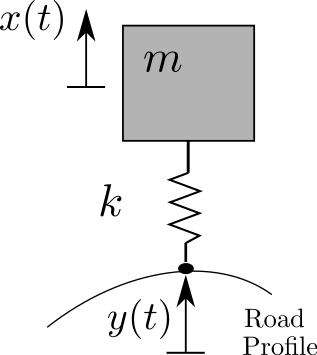
\includegraphics[scale=.5]{quarter_car_1dof_01.png} \vspc

\large The EOM is:\vspc

	\scalebox{1.0}{$m\ddot{x} +k(x-y)=0$} \vspc
	%\scalebox{1.0}{$ x(t=0)=x_0$\hspc and}\vspc
%	\scalebox{1.0}{$v(t=0)=v_0$}\vspc
\end{multicols}

}

\subsection{ State Space Model }
\frame{
\frametitle{ State Space Model }


\large The mass-spring system equation of motion can easily be written as a state space system.\vspc


\large  Equation of Motion:\vspc

	\scalebox{1.0}{$m\ddot{x}+k(x-y)=0$} \vspc \scalebox{1}{$z_1=x$\hspc and \hspc$z_2=\dot{x}$}\vspc
	\scalebox{1.0}{$\dot{z}_2=-\frac{k}{m}z_1+\frac{k}{m}y\hspc and \hspc\dot{z}_1=z_2$}\vspc

\[
\begin{bmatrix}
\dot{z}_{1} \\
\dot{z}_{2}
\end{bmatrix}
=
\begin{bmatrix}
0& 1\\
-\frac{k}{m} & 0
\end{bmatrix}
\begin{bmatrix}
z_1\\
z_2
\end{bmatrix}
+
\begin{bmatrix}
0\\
\frac{k}{m}
\end{bmatrix}
y(t)
\]

}

% Section 2: Mass Spring System Damper with Displacement Input
\section{Mass Spring System Damper with Displacement Input}

\subsection{Mass Spring Damper Model}
\frame{
\frametitle{Mass Spring Damper Model}

\begin{multicols}{2}
\large Consider the mass-spring system with damping now.\vspc

			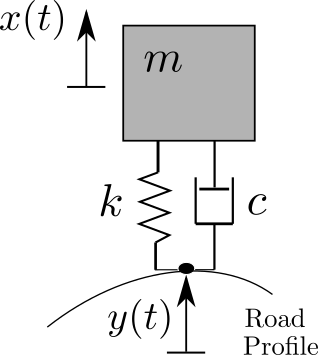
\includegraphics[scale=.5]{quarter_car_1dof_02.png} \vspc

\large The EOM is:\vspc

	\scalebox{1.0}{$m\ddot{x} +c(\dot{x}-\dot{y})+k(x-y)=0$} \vspc
	%\scalebox{1.0}{$ x(t=0)=x_0$\hspc and}\vspc
%	\scalebox{1.0}{$v(t=0)=v_0$}\vspc
\end{multicols}

}

\subsection{ State Space Model - Problem! }
\frame{
\frametitle{ State Space Model - Problem! }


\large The mass-spring system equation of motion cannot be written as a state space system easily this time.\vspc


\large  Equation of Motion:\vspc

	\scalebox{1.0}{$m\ddot{x}+c(\dot{x}-\dot{y})+k(x-y)=0$} \vspc \scalebox{1}{$z_1=x$\hspc and \hspc$z_2=\dot{x}$}\vspc
	\scalebox{1.0}{$\dot{z}_2=-\frac{c}{m}z_2+\frac{c}{m}\dot{y}-\frac{k}{m}z_1+\frac{k}{m}y\hspc and \hspc\dot{z}_1=z_2$}\vspcc

\large The $\dot{y}$ term is a problem! 
}

\subsection{ State Space Model - Fixed}
\frame{
\frametitle{ State Space Model - Fixed}


\large If we make a very clever substitution we can avoid this issue.\vspc


\large Equation of Motion:\vspc

	\scalebox{1.0}{$m\ddot{x}+c(\dot{x}-\dot{y})+k(x-y)=0$} \vspc \scalebox{1}{$z_1=x$\hspc and \hspc$z_2=\dot{x}-\frac{c}{m}y$}\vspc
	\scalebox{1.0}{$\dot{z}_2=-\frac{c}{m}(z_2+\frac{c}{m}y)-\frac{k}{m}z_1+\frac{k}{m}y\hspc and \hspc\dot{z}_1=z_2+\frac{c}{m}y$}\vspc
\[
\begin{bmatrix}
\dot{z}_{1} \vspace{3mm}\\
\dot{z}_{2}
\end{bmatrix}
=
\begin{bmatrix}
0& 1\vspace{3mm}\\
-\frac{k}{m} & -\frac{c}{m}
\end{bmatrix}
\begin{bmatrix}
z_1\vspace{3mm}\\
z_2
\end{bmatrix}
+
\begin{bmatrix}
\frac{c}{m}\vspace{3mm}\\
-(\frac{c}{m})^2+\frac{k}{m}
\end{bmatrix}
y(t)
\]

}

\subsection{ State Space Model - Output Equation }
\frame{
\frametitle{ State Space Model - Output Equation}


\large It is important that you keep the same substitutions when writing the output equations.\vspc

Output 1 - Position:\hspc \scalebox{1}{$y_{O1}=x=z_1$}\vspc

Output 2 - Velocity:\hspc \scalebox{1}{$y_{O2}=\dot{x}=\dot{z}_1=z_2+\frac{c}{m}y$}\vspc

\[
\begin{bmatrix}
\dot{y}_{O1} \vspace{3mm}\\
\dot{z}_{O2}
\end{bmatrix}
=
\begin{bmatrix}
1& 0\vspace{3mm}\\
0 & 1
\end{bmatrix}
\begin{bmatrix}
z_1\vspace{3mm}\\
z_2
\end{bmatrix}
+
\begin{bmatrix}
0\vspace{3mm}\\
\frac{c}{m}
\end{bmatrix}
y(t)
\]

}

% references is not a section for now, for looks and it would be a waste of space
\frame{

\frametitle{References}

\begin{itemize}
	\item System Dynamics, Palm III, Third Edition - Section 5.? - State Variable Models
\end{itemize}

}
\end{document}









 